\documentclass[a4paper,12pt]{report}
\usepackage{fontspec}
\setmainfont{Times New Roman}
\usepackage[russian]{babel}
\usepackage{amsmath}
\usepackage{graphicx}
\usepackage{geometry}
\usepackage{hyperref}
\usepackage{float}     % Для [H]
\usepackage{adjustbox} % Авто-масштабирование
\geometry{left=3cm,right=1.5cm,top=2cm,bottom=2cm}
\usepackage{setspace}
\onehalfspacing
\linespread{1.5}
\setlength{\parindent}{1.25cm}

\title{%
  \begin{center}
    
\includegraphics{../assets/gerb.png}
  \end{center}
  {\large МИНИСТЕРСТВО НАУКИ И ВЫСШЕГО ОБРАЗОВАНИЯ РОССИЙСКОЙ
  ФЕДЕРАЦИИ}\\[0.3cm]
  {\normalsize Федеральное государственное бюджетное образовательное
  учреждение высшего образования}\\[0.2cm]
  {\large \textbf{«МИРЭА --- Российский технологический университет»}}\\[0.1cm]
  {\normalsize РТУ МИРЭА}\\[0.3cm]
  {\normalsize Институт искусственного интеллекта (ИИИ)}\\
  {\normalsize Кафедра Промышленной информатики (ПИ)}\\[1cm]
  {\LARGE \textbf{ОТЧЕТ}}\\[0.2cm]
  {\Large \textbf{ПО ПРАКТИЧЕСКОЙ РАБОТЕ № 10}}\\[0.4cm]
  {\large \textbf{по дисциплине «Информатика»}}
}
\author{%
  \begin{tabular}{ll}
    Выполнил студент группы & КВБО-11-25 \\
    Принял ассистент        & Беднов Г.А. \\
  \end{tabular}
}
\date{%
  Практическую работу выполнил «10» 03 2026 г.\\[0.3cm]
  «Зачтено» «»  2026 г.\\[1cm]
  Москва 2026
}

\begin{document}
\maketitle

\noindent\textbf{Тема:} «Комбинационные устройства»\\
\noindent\textbf{Цель работы:} \\
• изучение  функциональных
характеристик  основных  комбинационных устройств (КУ);  \\
• освоение построения логических схем с КУ.
\begin{figure}[H]
  \centering
  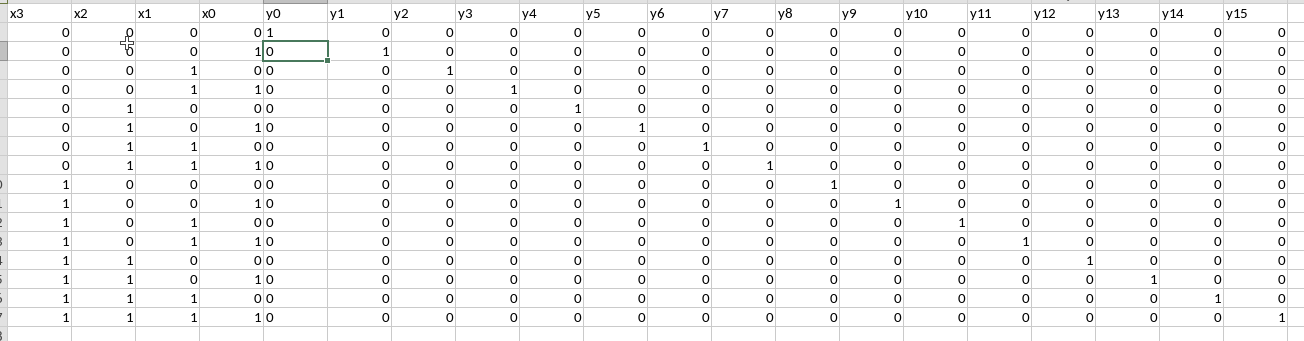
\includegraphics[width=\textwidth]{../assets/дешифратор.png}
  \caption{таблица дешифратора}
\end{figure}

\textbf{Логические уравнения дешифратора:}

\begin{align*}
  Y_0 &= \overline{X_3} \cdot \overline{X_2} \cdot \overline{X_1}
  \cdot \overline{X_0} \\
  Y_1 &= \overline{X_3} \cdot \overline{X_2} \cdot \overline{X_1}
  \cdot X_0 \\
  Y_2 &= \overline{X_3} \cdot \overline{X_2} \cdot X_1 \cdot
  \overline{X_0} \\
  Y_3 &= \overline{X_3} \cdot \overline{X_2} \cdot X_1 \cdot X_0 \\
  Y_4 &= \overline{X_3} \cdot X_2 \cdot \overline{X_1} \cdot
  \overline{X_0} \\
  Y_5 &= \overline{X_3} \cdot X_2 \cdot \overline{X_1} \cdot X_0 \\
  Y_6 &= \overline{X_3} \cdot X_2 \cdot X_1 \cdot \overline{X_0} \\
  Y_7 &= \overline{X_3} \cdot X_2 \cdot X_1 \cdot X_0 \\
  Y_8 &= X_3 \cdot \overline{X_2} \cdot \overline{X_1} \cdot
  \overline{X_0} \\
  Y_9 &= X_3 \cdot \overline{X_2} \cdot \overline{X_1} \cdot X_0 \\
  Y_{10} &= X_3 \cdot \overline{X_2} \cdot X_1 \cdot \overline{X_0} \\
  Y_{11} &= X_3 \cdot \overline{X_2} \cdot X_1 \cdot X_0 \\
  Y_{12} &= X_3 \cdot X_2 \cdot \overline{X_1} \cdot \overline{X_0} \\
  Y_{13} &= X_3 \cdot X_2 \cdot \overline{X_1} \cdot X_0 \\
  Y_{14} &= X_3 \cdot X_2 \cdot X_1 \cdot \overline{X_0} \\
  Y_{15} &= X_3 \cdot X_2 \cdot X_1 \cdot X_0
\end{align*}

\begin{figure}[H]
  \centering
  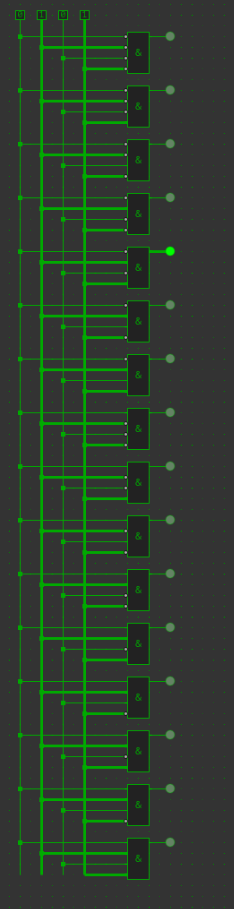
\includegraphics[width=0.3\textwidth]{../assets/схема дешифратора.png}
  \caption{схема дешифратора}
  \label{fig:схема-дешифратора}
\end{figure}

Уменьшить логическую схему не получится так как каждое уравнение
состоит из одной конъюнкции.

\begin{figure}[H]
  \centering
  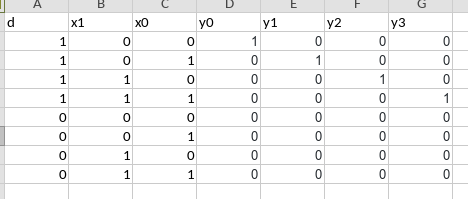
\includegraphics[width=0.8\textwidth]{../assets/2026-03-09-15-44-46.png}
  \caption{демультиплексор}
  \label{fig:2026-03-09-15-44-46}
\end{figure}

\begin{figure}[H]
  \centering
  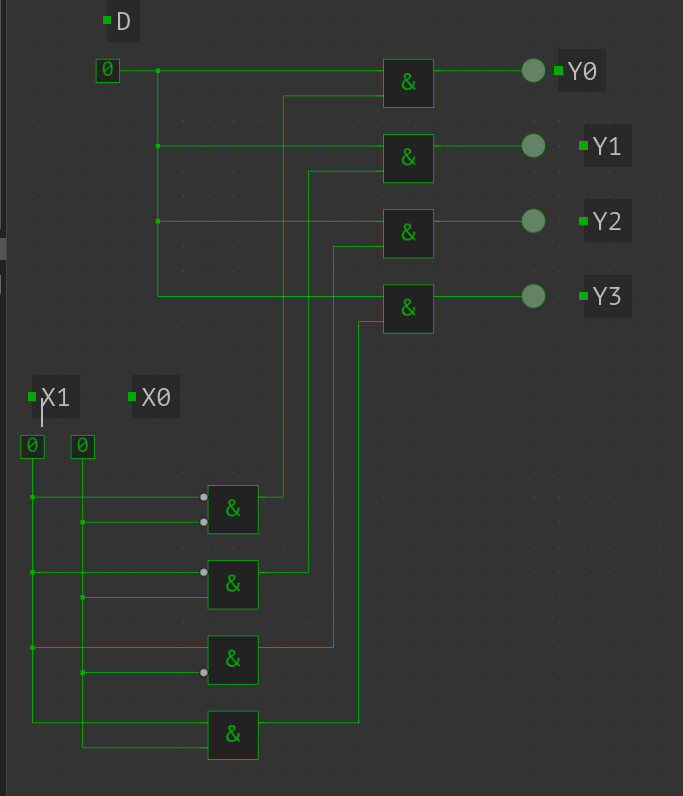
\includegraphics[width=0.8\textwidth]{../assets/схема демультиплексора.png}
  \caption{схема демультиплексора}
  \label{fig:схема-демультиплексора}
\end{figure}

\begin{figure}[H]
  \centering
  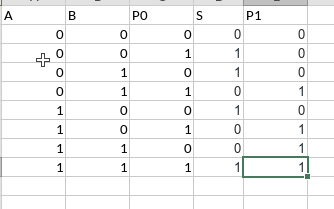
\includegraphics[width=0.8\textwidth]{../assets/таблица сумматора.png}
  \caption{таблица сумматора}
  \label{fig:таблица-сумматора}
\end{figure}

\begin{figure}[H]
  \centering
  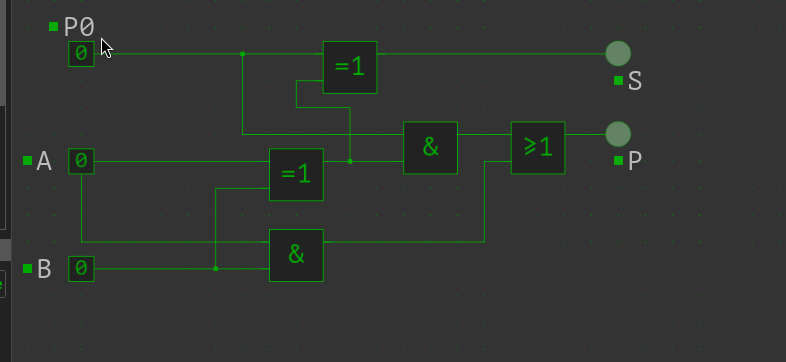
\includegraphics[width=0.8\textwidth]{../assets/сумматор.png}
  \caption{схема сумматора}
  \label{fig:сумматор}
\end{figure}

\textbf{Логические уравнения:}
\begin{gather*}
  S = \overline{A} \cdot \overline{B} \cdot P_0 + \overline{A}
  \cdot B \cdot \overline{P_0} + A \cdot \overline{B} \cdot
  \overline{P_0} + A \cdot B \cdot P_0 \\
  P_{i+1} = \overline{A} \cdot B \cdot P_0 + A \cdot
  \overline{B} \cdot P_0 + A \cdot B \cdot \overline{P_0} + A
  \cdot B \cdot P_0
\end{gather*}

\end{document}
